
\documentclass[hyperref={pdfpagelabels=false},ngerman]{beamer}

% stop font warning
\let\Tiny=\tiny
\providecommand\thispdfpagelabel[1]{}

\usepackage[english]{babel}
\usepackage{lmodern}
\usepackage[T1]{fontenc}
\usepackage[utf8]{inputenc}
\usepackage{graphicx,import}
\usepackage{feynmp}
\DeclareGraphicsRule{*}{mps}{*}{} 
\DeclareGraphicsExtensions{.pdf}
\usepackage{amsmath,amssymb,amstext,amsfonts} % mathrsfs
\usepackage{array,booktabs,tabularx}
\usepackage{tikz,tikz-uml,pgf-pie}
\usetikzlibrary{shapes,calc,arrows,positioning,shapes}
\tikzstyle{block} = [rectangle, draw, thick, text width=10em, text centered, minimum height=2em]
\tikzstyle{arrow} = [draw, -latex, thick]
\tikzstyle{arrow2} = [draw, latex-latex, thick]
\tikzstyle{quark}  = [rectangle, draw, fill=yellow, minimum width=2em, text centered, minimum height=2em]
\tikzstyle{lepton} = [rectangle, draw, fill=red!50, minimum width=2em, text centered, minimum height=2em]
\tikzstyle{gauge}  = [circle   , draw, fill=green , minimum size=2em, inner sep=0pt, text centered]
\tikzstyle{scalar} = [diamond  , draw, fill=blue!40, minimum width=2.3em, text centered, minimum height=2.3em, inner sep=0pt]
\tikzstyle{goldstone} = [diamond, draw, dashed, fill=blue!30, minimum width=2.3em, text centered, minimum height=2.3em, inner sep=0pt]
\tikzstyle{squark}   = [diamond, draw, fill=yellow, minimum width=2.3em, text centered, minimum height=2.3em, inner sep=0pt]
\tikzstyle{slepton}  = [diamond, draw, fill=red!50, minimum width=2.3em, text centered, minimum height=2.3em, inner sep=0pt]
\tikzstyle{gaugino}  = [rectangle, draw, fill=green , minimum size=2em, inner sep=0pt, text centered]
\tikzstyle{higgsino} = [rectangle, draw, fill=blue!40  , minimum width=2em, text centered, minimum height=2em]
\tikzstyle{inert}    = [diamond  , draw, fill=teal!80, minimum width=2.3em, text centered, minimum height=2.3em, inner sep=0pt]
\tikzstyle{inertino} = [rectangle, draw, fill=teal!80, minimum width=2em, text centered, minimum height=2em]
\tikzstyle{phantom}  = [rectangle, minimum width=2em, text centered, minimum height=2em]
\usepackage{slashed}
\usepackage{fixltx2e} % textsubscript
\usepackage{multirow}
\usepackage{tcolorbox}
\usepackage{pifont}
\usepackage{xspace}
\usepackage{hyperref}
\hypersetup{colorlinks,linkcolor=,urlcolor=blue}
\usepackage{listings}
\lstset{breaklines=true,
  breakatwhitespace=true,
%  numbers=left,
  numberstyle=\tiny,
  stepnumber=1,
  basicstyle=\ttfamily\footnotesize,
  commentstyle=\ttfamily\color{gray},
  postbreak={\mbox{{$\hookrightarrow$}}\space\space},
  breakindent=10pt,
  breakautoindent=false,
  showspaces=false,
  showstringspaces=false,
  frame=single}

\definecolor{darkgreen}{RGB}{0,176,0}

\newcommand{\cmark}{\ding{51}}%
\newcommand{\xmark}{\ding{55}}%
\newcommand{\fmfvcenter}[1]{\;\vcenter{\hbox{\fmfreuse{#1}}}\;}
\newcommand{\eh}[1]{\,\mathsf{#1}}
\newcommand{\ok}{\textcolor{darkgreen}{\cmark}}
\newcommand{\notok}{\textcolor{red}{\xmark}}
\newcommand{\maybe}{\textcolor{gray}{\cmark}}
\newcommand{\meh}{\textcolor{gray}{\textbf{\huge\lower.1em\hbox{-}}}}
\newcommand{\Lagr}{\mathcal{L}}
\newcommand{\MS}{\ensuremath{M_S}}
\newcommand{\mathi}{\mathsf{i}}
\newcommand{\mycite}[1]{\ensuremath{\text{\textcolor{darkgray}{\tiny [#1]}}}}
\newcommand{\bigcite}[1]{\textcolor{darkgray}{[#1]}}
\newcommand{\dimrep}[1]{\mathbf{#1}}
\newcommand{\dimrepadj}[1]{\mathbf{\overline{#1}}}
\newcommand{\ESSM}{E\textsubscript{6}SSM}
\newcommand{\CESSM}{CE\textsubscript{6}SSM}
\DeclareMathOperator{\tildeRe}{\widetilde Re}
\DeclareMathOperator{\sign}{sign}
\DeclareMathOperator{\re}{Re}
\DeclareMathOperator{\im}{Im}
\renewcommand{\emph}{\textbf}
\newcommand{\dd}{\mathsf{d}}
\newcommand{\myurl}[1]{\href{#1}{#1}}
\newcommand{\Superpot}{\mathcal{W}}
\newcommand{\SuperField}[1]{#1}
\newcommand{\ConjSuperField}[1]{\bar{#1}}
\newcommand{\UY}{\ensuremath{U(1)_{Y}}}
\newcommand{\UN}{\ensuremath{U(1)_{N}}}
\newcommand{\Uem}{\ensuremath{U(1)_\text{em}}}
\newcommand{\SUL}{\ensuremath{SU(2)_\text{L}}}
\newcommand{\SUc}{\ensuremath{SU(3)_\text{c}}}
\newcommand{\SOten}{\ensuremath{{SO(10)}}}
\newcommand{\comma}{,}
\newcommand{\DRbar}{\ensuremath{\overline{\text{DR}}}}
\newcommand{\MSbar}{\ensuremath{\overline{\text{MS}}}}
\newcommand{\SM}{\ensuremath{\text{SM}}}
\newcommand{\MSSM}{\ensuremath{\text{MSSM}}}
\newcommand{\pole}{\ensuremath{\text{pole}}}
\newcommand{\tree}{\ensuremath{\text{tree}}}
\newcommand{\fsstar}{\textbf{*}}
\newcommand{\Zv}{\ensuremath{\backslash\mkern-11.0mu{Z_3}}}
\newcommand{\downrightknickarrow}{\mathrel{\scalebox{1.3}{\rotatebox[origin=c]{180}{$\Lsh$}}}}
\newcommand{\threelinebrace}{$\left. \begin{array}{c} \\ \\ \\ \end{array} \right\rbrace$}
\newcommand{\fivelinebrace}{$\left. \begin{array}{c} \\ \\ \\ \\ \\ \end{array} \right\rbrace$}
\newcommand{\twolinebrace}{$\left. \begin{array}{c} \\ \\ \end{array} \right\rbrace$}
\newcommand{\elevenlinebrace}{$\left. \begin{array}{c} \\ \\ \\ \\ \\ \\ \\ \\ \\ \\ \\ \end{array} \right\rbrace$}
\newcommand{\at}{\alpha_t}
\newcommand{\ab}{\alpha_b}
\newcommand{\atau}{\alpha_\tau}
\newcommand{\as}{\alpha_s}
\newcommand{\SARAH}{\texttt{SARAH}}
\newcommand{\Mathematica}{\texttt{Mathematica}}
\newcommand{\Himalaya}{\texttt{Himalaya}}
\newcommand{\GMTCalc}{\texttt{GM2Calc}}

% set look of slides
\usetheme{Madrid}
\useoutertheme{default}
\useinnertheme{circles}
\usecolortheme{default}
\beamertemplatenavigationsymbolsempty % keine Navigationselemente
\setbeamersize{text margin left = 1cm, text margin right = 1cm}

% define footer
\makeatletter
\setbeamertemplate{footline}
{
  \hfill\hbox{\insertframenumber{} / \inserttotalframenumber\hspace*{4pt}}%
  \vskip3pt%
}
\makeatother
\usecolortheme{tud}

\title{FlexibleSUSY}

\author[Alexander Voigt]{Alexander Voigt\\[0.5em]{\small In
    collaboration with P.\ Athron, M.\ Bach, D.\ Harries, T.\
    Kwasnitza, J.-h.\ Park, D.\ Stöckinger, J.\ Ziebell}}

\date{GAMBIT webinar, 27.10.2017}

\institute[Aachen]{RWTH Aachen}
\subject{FlexibleSUSY,MSSM,Higgs,FlexibleEFTHiggs}
\keywords{FlexibleSUSY,MSSM,Higgs,FlexibleEFTHiggs}

%%%%%%%%%%%%%%%%%%%%%%%%%%%%%%%%%%%%%%%%%%%%%%%%%%%%%%%%%%%%%%%%%%%%%%%%%%%%%

\begin{document}

%%%%%%%%%%%%%%%%%%%%%%%%%%%%%%%%%%%%%%%%
\begin{frame}[plain]
  \tikz [remember picture,overlay]
  \node at
    ([yshift=1.3cm,xshift=4cm]current page.south)
    {\includegraphics[height=2cm]{images/RWTH_Logo}};
  \tikz [remember picture,overlay]
  \node at
    ([yshift=2cm,xshift=-4cm]current page.south)
    {\includegraphics[height=2.5cm]{images/FS.png}};
  \titlepage  
\end{frame}

%%%%%%%%%%%%%%%%%%%%%%%%%%%%%%%%%%%%%%%%
\begin{frame}{Contents}
  \tableofcontents
\end{frame}

\section{What is FlexibleSUSY?}

\begin{frame}{What is FlexibleSUSY?}
  \begin{center}
    \includegraphics[width=\textwidth]{images/FS.png}
  \end{center}
\end{frame}

\begin{frame}{What is FlexibleSUSY?}
  \begin{center}
    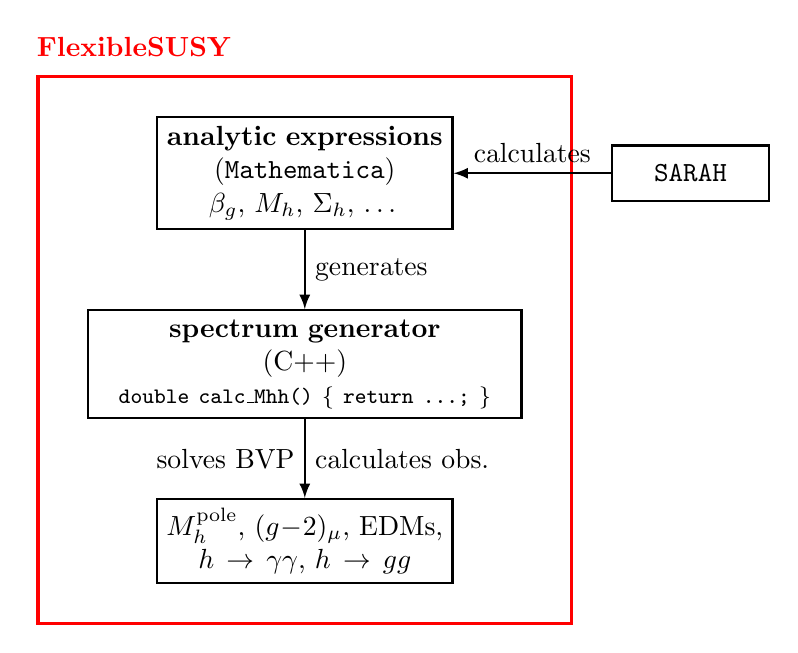
\begin{tikzpicture}
    \node[block] (EXPR) {\textbf{analytic expressions}\\ (\Mathematica)\\ $\beta_g$, $M_h$, $\Sigma_h$, \ldots};
    % \node[block, below = 1cm of EXPR, text width=15em] (FS) {\textbf{spectrum generator}\\ (C++)\\ solves BVP, calculates observables};
    \node[block, below = 1cm of EXPR, text width=15em] (FS) {\textbf{spectrum generator}\\ (C++)\\ \footnotesize{\texttt{double calc\_Mhh() \{ return ...; \}}}};
    \node[block, below = 1cm of FS] (OUT) {$M_h^\pole$, $(g-2)_\mu$, EDMs, $h\rightarrow\gamma\gamma$, $h\rightarrow gg$};
    \path[arrow] (EXPR) -- node[right]{generates} (FS);
    \path[arrow] (FS) -- node[right]{calculates obs.} node[left]{solves BVP} (OUT);
    \draw[red,very thick] ($(EXPR.north west)+(-1.5,0.5)$) node(FSname){} rectangle ($(OUT.south east)+(1.5,-0.5)$);
    \node[above right = 0cm and 0cm of FSname.north west] {\textbf{\textcolor{red}{FlexibleSUSY}}};
    \node[block, right = 2cm of EXPR, text width=5em] (SARAH) {\textbf{\SARAH}};
    \path[arrow] (SARAH) -- node[above]{calculates} (EXPR);
    \end{tikzpicture}
  \end{center}
\end{frame}

\begin{frame}{Example: CMSSM}
  \begin{center}
  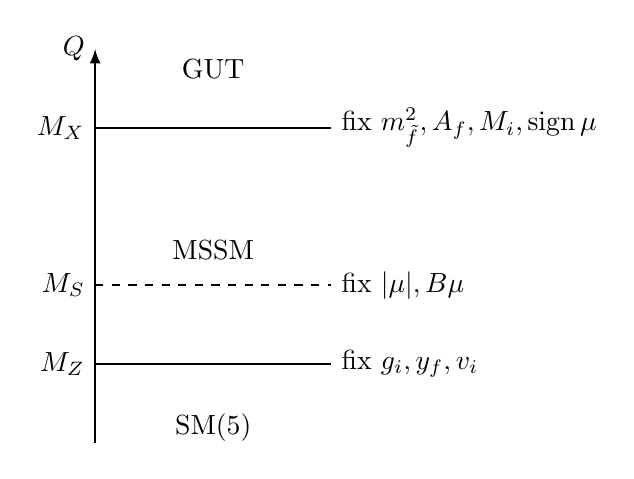
\begin{tikzpicture}
    \path[arrow] (0,0) -- (0,5) node[left]{$Q$};
    \draw[thick] (0,4) node[left]{$M_X$} -- node[above = 0.5cm]{GUT} (3,4) node[right]{fix $m_{\tilde{f}}^2, A_f, M_i, \sign\mu$};
    \draw[thick,dashed] (0,2) node[left]{$M_S$} -- (3,2) node[right]{fix $|\mu|, B\mu$};
    \draw[thick] (0,1) node[left]{$M_Z$} -- node[above = 1.2cm]{MSSM} node[below = 0.5cm]{SM(5)} (3,1) node[right]{fix $g_i, y_f, v_i$};
  \end{tikzpicture}
  \end{center}
\end{frame}

\begin{frame}{Example: CNMSSM}
  \begin{center}
  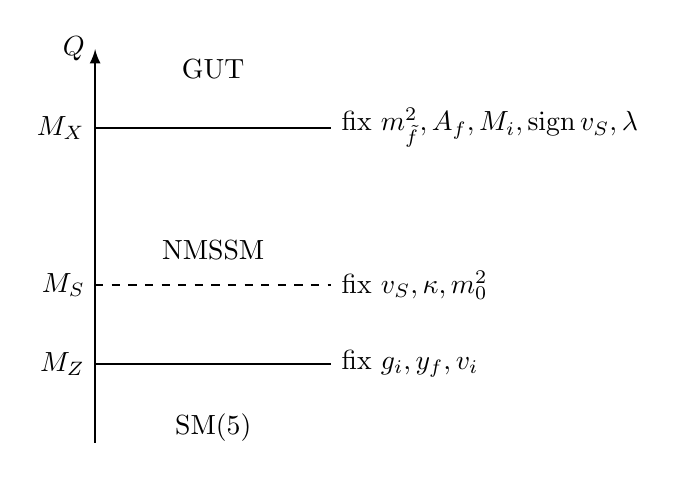
\begin{tikzpicture}
    \path[arrow] (0,0) -- (0,5) node[left]{$Q$};
    \draw[thick] (0,4) node[left]{$M_X$} -- node[above = 0.5cm]{GUT} (3,4) node[right]{fix $m_{\tilde{f}}^2, A_f, M_i, \sign v_S, \lambda$};
    \draw[thick,dashed] (0,2) node[left]{$M_S$} -- (3,2) node[right]{fix $v_S, \kappa, m_0^2$};
    \draw[thick] (0,1) node[left]{$M_Z$} -- node[above = 1.2cm]{NMSSM} node[below = 0.5cm]{SM(5)} (3,1) node[right]{fix $g_i, y_f, v_i$};
  \end{tikzpicture}
  \end{center}
\end{frame}

\begin{frame}{Example: HSSUSY}
  \begin{center}
  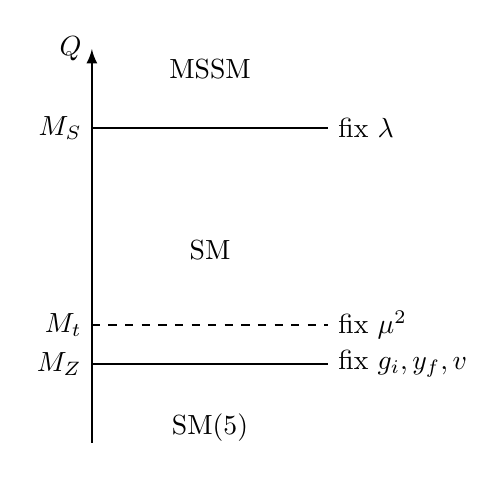
\begin{tikzpicture}
    \path[arrow] (0,0) -- (0,5) node[left]{$Q$};
    \draw[thick] (0,4) node[left]{$M_S$} -- node[above = 0.5cm]{MSSM} (3,4) node[right]{fix $\lambda$};
    \draw[thick,dashed] (0,1.5) node[left]{$M_t$} -- (3,1.5) node[right]{fix $\mu^2$};
    \draw[thick] (0,1) node[left]{$M_Z$} -- node[above = 1.2cm]{SM} node[below = 0.5cm]{SM(5)} (3,1) node[right]{fix $g_i, y_f, v$};
  \end{tikzpicture}
  \end{center}
\end{frame}

\section{Features}

\begin{frame}{Features for all models}
  Physics features:
  \begin{itemize}
  \item calculation in the \MSbar/\DRbar\ scheme
  \item real or complex parameters
  \item 2-loop running (RGEs from \SARAH)
  \item 1-loop threshold corrections
  \item 1-loop pole masses (1-loop corrections from \SARAH)
  \item 1-loop $(g-2)_\mu$ + 2-loop leading QED log
  \item 1-loop EDMs for all fundamental fermions
  \item effective couplings $h\rightarrow \gamma\gamma$ and
    $h\rightarrow gg$ at N$^3$LO QCD
  \item 1-loop $M_W$ prediction from $G_F$ + 2-loop SM contributions
  \item 1-loop FlexibleEFTHiggs calculation of $M_h$
  \end{itemize}
  %
  Non-physics features:
  \begin{itemize}
    \item SLHA input/output
    \item \Mathematica\ input/output
    \item SQL database output
    \item modular C++ code
  \end{itemize}
\end{frame}

\begin{frame}{Model-specific higher order contributions}
  \emph{SM:}
  \begin{itemize}
  \item 3-loop running
  \item 3-loop QCD threshold corrections to $y_t$, $y_b$, $\alpha_s$
  \item 3-loop contributions to $M_h$
  \item 2-loop threshold corrections to the MSSM (\texttt{HSSUSY})
  \end{itemize}
  \emph{MSSM:}
  \begin{itemize}
  \item 3-loop running
  \item 2-loop SQCD threshold corrections to $y_t$, $y_b$, $\alpha_s$
  \item 2-loop contributions to $M_{h,H,A}$
  \item 3-loop contributions to $M_h$ (via \Himalaya)
  \item 2-loop $(g-2)_\mu$ (via \GMTCalc)
  \end{itemize}
  \emph{NMSSM:}
  \begin{itemize}
  \item skipping \ldots
  \end{itemize}
  % \begin{itemize}
  % \item 2-loop SQCD threshold corrections to $y_t$, $y_b$, $\alpha_s$
  % \item 2-loop contributions to $M_{h,H,A}$
  % \end{itemize}
  \emph{split-MSSM:}
  \begin{itemize}
  \item skipping \ldots
  \end{itemize}
  % \begin{itemize}
  % \item 2-loop QCD threshold corrections to $y_t$, $y_b$, $\alpha_s$
  % \item 3-loop contributions to $M_h$
  % \item 2-loop threshold corrections to the MSSM (\texttt{SplitMSSM})
  % \end{itemize}
  \emph{THDM-II:}
  \begin{itemize}
  \item skipping \ldots
  \end{itemize}
\end{frame}

\section{Example: HSSUSY}

\begin{frame}{Example: HSSUSY}
  hands-on example
\end{frame}

\end{document}
